\part{Mecánica Cuántica}

\vspace*{\fill}

\begin{center}
	\textit{''Cualquiera que no se sorprenda por la teoría cuántica, no la ha entenddo'' - Niels Bohr.}
\end{center}

\vspace*{\fill}


\chapter{Notación de Dirac (Repaso Álgebra Lineal)}

Se hará un repaso de ciertas definiciones y propiedades, para tenerlas frescas, no se ahondará demasiado en cada una, ni se demostrarán. \\


\section{Espacios de Hilbert y Espacio Dual}
Los estados en mecánica Cuántica son descritos por medio de vectores. Sea $\hilbert$ un espacio vectorial sobre un campo escalar $\F$, pero en Mecánica Cuántica el campo de escalares es el campo de los números complejos $\C$. Los elementos de $\hilbert$ son vectores. Si $\phi \in \hilbert$, en la notación de Dirac lo escribimos de la siguiente forma
	$$ \phi = \ket{\phi} \qquad \text{Kets}. $$
	
Los elementos de $\hilbert$ los llamamos, vectores o kets. De esta forma decios que el ket $\ket{\phi} \in \hilbert$. Si $\lambda$ es un escalar, o sea que $\lambda \in \C$ la multiplicación por escalar queda así $\lambda \phi = \ket{\lambda \phi} = \lambda \ket{\phi} \in \hilbert$.

\subsection{El Espacio Dual}
Sea $\hilbert ^*$ el espacio dual albegraico de $\hilbert$. La definición de $\hilbert ^*$ es la siguiente: $\hilbert ^* = \{ \psi : \hilbert \to \C \text{ tal que } \psi \text{ es lineal} \}$. A $\psi$ se le conoce como funcional o Bra. Los cuales son descritos de la siguiente forma $\psi \in \hilbert ^*$ entonces $\psi = \bra{\psi}$. Una propiedad importante de esto que mencionamos es que a todo Ket le corresponde un Bra. En la notación de Dirac el funcional $\psi \in \hilbert ^*$ operando sobre el ket $\phi \in \hilbert$ se escribe de la siguiente manera
	$$ \psi (\phi) = \braket{\psi}{\phi} \in \C \qquad \text{Braket}. $$

\section{Operadores Lineales}
Sea $\hilbert$ un espacio vectorial sobre $\F$. Una función $A:\hilbert \to \hilbert$ es un operador lineal si y solo si para todos $2$ vectores cualesquiera del espacio y un escalar de campo $A(\phi _1 + \phi _2) = A\phi_1 + A\phi _2$ y $A(\lambda \phi _1) = \lambda A \phi_1$. Los cuales son representados por matrices. Dado que los Bra son lineales, cumplen con estas características, es decir que los brakets son lineales en la segunda coordenada \dsnote{la parte del ket}. En Mecánica Cuántica usaremos operadores hermíticos, unitarios y escalares. Cuando un operador actua sobre un braket se escribe de la siguiente forma $\mel{\psi}{A}{\phi}$.


\section{Los KetBras}
Sea $\hilbert$ un espacio vectorial sobre los números complejos y $\hilbert ^*$ es su espacio dual. Para todo $\ket{\phi} \in \hilbert$ y todo bra $\bra{\psi} \in \hilbert ^*$, definimos el ketbra $\ketbra{\phi}{\psi}$ de la siguiente forma
	$$ \ketbra{\phi}{\psi}:\hilbert \to \hilbert $$
	$$ \ket{\alpha} \mapsto \ket{\beta} = \braket{\psi}{\beta} \ket{\phi} $$
Esto es bastante confuso viendo solo así, el resto de operaciones son bastante intuitivas o ya conocidas, pero esta es un producto tensorial conocido como \textbf{producto exterior} calculado de la siguiente forma \dsnote{no se ha mencionado pero es bastante obvio, los kets son vectores columna y los bra vectores fila}.
	$$ \ketbra{\phi}{\psi} = \mqty(\phi_1 \\ \phi_2 \\ \vdots \\ \phi _N) \mqty(\psi _1 & \psi _2 & \cdots \psi _N) = \mqty( \phi _1 \psi_1 & \phi _1 \psi_2 & \cdots & \phi _1 \psi _N \\
						 \phi _2 \psi_1 & \phi _2 \psi_2 & \cdots & \phi _2 \psi _N \\
						 \vdots & \vdots &\ddots & \vdots \\
						 \phi _N \psi_1 & \phi _N \psi_2 & \cdots & \phi _N \psi _N \\ ) $$
Esto no se vio en clase pero es imprescindible saberlo. Además, uno de los usos de esto es la construcción de un operador de proyección, dado un ket de norma 1, la proyección ortonormal en el subespacio generado por $\ket{\phi}$ es $\ketbra{\phi}$. Este es un operador idempotente\footnote{Un operador idempotente es uno que aplicado sobre sí mismo da como resultado él mismo, $A^2 = A$.} \\

\subsection{Producto de kronecker}
El producto tensorial de Kronecker es el que utilizaremos en mecánica cuántica (el producto de Kronecker es una generalización a matrices del producto exterior)
%    $$ \mathbf{A} \otimes \mathbf{B} =
%            \begin{bmatrix}
%            \phi_{11} \mathbf{B} & \phi_{12} \mathbf{B} & \phi_{13} \mathbf{B} \\
%            \phi_{21} \mathbf{B} & \phi_{22} \mathbf{B} & \phi_{23} \mathbf{B} \\
%            \phi_{31} \mathbf{B} & \phi_{32} \mathbf{B} & \phi_{33} \mathbf{B}
%            \end{bmatrix} =
%            \begin{bmatrix}
%            \phi_{11}\psi_{11} & \phi_{11}\psi_{12} & \phi_{12}\psi_{11} & \phi_{12}\psi_{12} & \phi_{13}\psi_{11} & \phi_{13}\psi_{12} \\
%            \phi_{11}\psi_{21} & \phi_{11}\psi_{22} & \phi_{12}\psi_{21} & \phi_{12}\psi_{22} & \phi_{13}\psi_{21} & \phi_{13}\psi_{22} \\
%            \phi_{21}\psi_{11} & \phi_{21}\psi_{12} & \phi_{22}\psi_{11} & \phi_{22}\psi_{12} & \phi_{23}\psi_{11} & \phi_{23}\psi_{12} \\
%            \phi_{21}\psi_{21} & \phi_{21}\psi_{22} & \phi_{22}\psi_{21} & \phi_{22}\psi_{22} & \phi_{23}\psi_{21} & \phi_{23}\psi_{22} \\
%            \phi_{31}\psi_{11} & \phi_{31}\psi_{12} & \phi_{32}\psi_{11} & \phi_{32}\psi_{12} & \phi_{33}\psi_{11} & \phi_{33}\psi_{12} \\
%            \phi_{31}\psi_{21} & \phi_{31}\psi_{22} & \phi_{32}\psi_{21} & \phi_{32}\psi_{22} & \phi_{33}\psi_{21} & \phi_{33}\psi_{22}
%            \end{bmatrix} $$


    $$ \mathbf{A} \otimes \mathbf{B} =
        \begin{bmatrix}
        \color{red}\phi_{11} \mathbf{B} & \color{blue}\phi_{12} \mathbf{B} & \color{green}\phi_{13} \mathbf{B} \\
        \color{orange}\phi_{21} \mathbf{B} & \color{purple}\phi_{22} \mathbf{B} & \color{cyan}\phi_{23} \mathbf{B} \\
        \color{magenta}\phi_{31} \mathbf{B} & \color{brown}\phi_{32} \mathbf{B} & \color{gray}\phi_{33} \mathbf{B}
        \end{bmatrix} =
        \begin{bmatrix}
        \color{red}\phi_{11}\psi_{11} & \color{red}\phi_{11}\psi_{12} & \color{blue}\phi_{12}\psi_{11} & \color{blue}\phi_{12}\psi_{12} & \color{green}\phi_{13}\psi_{11} & \color{green}\phi_{13}\psi_{12} \\
        \color{red}\phi_{11}\psi_{21} & \color{red}\phi_{11}\psi_{22} & \color{blue}\phi_{12}\psi_{21} & \color{blue}\phi_{12}\psi_{22} & \color{green}\phi_{13}\psi_{21} & \color{green}\phi_{13}\psi_{22} \\
        \color{orange}\phi_{21}\psi_{11} & \color{orange}\phi_{21}\psi_{12} & \color{purple}\phi_{22}\psi_{11} & \color{purple}\phi_{22}\psi_{12} & \color{cyan}\phi_{23}\psi_{11} & \color{cyan}\phi_{23}\psi_{12} \\
        \color{orange}\phi_{21}\psi_{21} & \color{orange}\phi_{21}\psi_{22} & \color{purple}\phi_{22}\psi_{21} & \color{purple}\phi_{22}\psi_{22} & \color{cyan}\phi_{23}\psi_{21} & \color{cyan}\phi_{23}\psi_{22} \\
        \color{magenta}\phi_{31}\psi_{11} & \color{magenta}\phi_{31}\psi_{12} & \color{brown}\phi_{32}\psi_{11} & \color{brown}\phi_{32}\psi_{12} & \color{gray}\phi_{33}\psi_{11} & \color{gray}\phi_{33}\psi_{12} \\
        \color{magenta}\phi_{31}\psi_{21} & \color{magenta}\phi_{31}\psi_{22} & \color{brown}\phi_{32}\psi_{21} & \color{brown}\phi_{32}\psi_{22} & \color{gray}\phi_{33}\psi_{21} & \color{gray}\phi_{33}\psi_{22}
        \end{bmatrix} $$


\section{Más Sobre Operadores Lienales}

\subsection{La Transpuesta}
Sea $A:\hilbert _1 \to \hilbert _2$ un operador lineal \dsnote{que no un operador es una transformación de un espacio sobre sí mismo??} donde $\hilbert _1$ y $\hilbert _2$ son espacios vectoriales sobre $\C$. Definimos la transpuesta de $A$, denotada por $A^T$, como
	$$ A^T : \hilbert _2 ^* \to \hilbert _1 ^* $$
	$$ \bra{\beta} \mapsto \bra{\alpha} = A^T (\bra{\beta}) $$
o sea que $A^T \bra{\beta} = \bra{\beta} A$.



\subsection{Bases y Bases Duales}

Sea $\hilbert$ un espacio vectorial sobre los complejos, y $\alpha = \{ \ket{\alpha_1},\ldots ,\ket{\alpha _k} \}$ base de $\hilbert$. La base dual de la siguiente forma $\beta = \{ \bra{\beta _1} ,\ldots ,\bra{\beta _k} \}$ donde
	$$ \boxed{ \braket{\beta _i}{\alpha _j} = \delta _{ij} = \left\{ \mqty{1 & \text{si} & i=j \\ 0 & \text{si} & i\neq j} \right. } $$




\section{Componentes de Kets y Bras}
Por definición de base todo elemento del espacio puede ser escrito como combinación lineal de la base. Con esto se tienen las siguientes propiedades
\begin{description}
	\item[Fourier en Abstracto: ] $a_i = \braket{\beta _i}{\phi}$. O de manera continua
		$$ \ket{\phi} = \int _{x\in \R} \dd{x} \phi (x) \ket{\alpha _x} $$
		con $\phi (x)$ función de onda.
	\item[Covarianza y contravarianza: ] Los kets son vectores contravariantes y los bras son vectores covariantes.
	\item[Fourier en Abstracto: ] $b_i = \braket{\psi}{\alpha _i}$. O de manera continua
		$$ \ket{\phi} = \int \dd{x} \phi (x) \ket{x}, $$
		$$ \bra{\psi} = \int \dd{x} \bra{x} \psi (x). $$
	\item[Representación matricial de operadores lineales: ] $a_{ij} = \mel{\beta _i}{T}{\alpha _j}$, $A$ es la representación matricial de $T$ respecto a la base $\alpha$.
		$$ T\ket{\alpha _j} = \sum _{k=1} ^n a_{kj} \ket{\alpha _k}. $$
\end{description}


\begin{teorema}
	Sea $T:\hilbert \to \hilbert$ un operador lineal y $\alpha = \{ \ket{\alpha _i} \}$ una base de $\hilbert$. Si $a_{ij} = \mel{\beta _i}{T}{\alpha _j}$ entonces
		$$ T = \sum_{i=1} ^n \sum _{j=1} ^n a_{ij} \ketbra{\alpha _i}{\beta _j}. $$
\end{teorema}


\begin{description}
	\item[La Identidad: ] La identidad $I:\hilbert \to \hilbert$ es un operador lineal que deja todo igual.
		$$ I = \sum_{i=1} ^n \ketbra{\alpha _i}{\beta _i}. $$
\end{description}



\section{Espacios de Hilbert}
Un espacio de HIlbert, como lo explicaremos más adelante, es un Espcio vectorial con producto interno completo\footnote{Es decir, que toda secuencia de Cauchy converge dentro del espacio.}.

\subsection{Produto Interno}
Sea $\hilbert$ un espacio vectorial sobre el campo de los números complejos $\C$. Un producto interno en $\hilbert$ es una función de la siguiente forma
	$$ \inner{\,}{\,}: \hilbert \times \hilbert \to \C $$

que tiene las siguientes propiedades
\begin{enumerate}
	\item Asimetría.
	\item Linealidad segunda componente.
	\item Definida positiva.
	\item No degenerado.
\end{enumerate}
La pareja $\qty(\hilbert ,\inner{\,}{\,})$ es llamada espacio con producto interno. 
\begin{description}
	\item[Primera Propiedad: ] $\inner{k\psi}{\phi} = k^* \inner{\psi}{\phi}$.
	\item[Segunda Propiedad: ] $\inner{\psi _1 + \psi _2}{\phi} = \inner{\psi _1}{\phi} + \inner{\psi _2}{\phi}$.
\end{description}

\subsubsection{Norma}
Sea $(\hilbert ,\inner{\,}{\,})$ un espacio con producto interno, para todo vector $\phi \in \hilbert$ se define la norma de $\phi$ de la siguiente forma
	$$ \norm{\phi} = \sqrt{\inner{\phi}{\phi}}. $$
\begin{description}
	\item[Tercera Propiedad: ] $\abs{\inner{\psi}{\phi}} \leq \norm{\psi}\norm{\phi}$.
	\item[Cuarta Propiedad: ] $\norm{\psi + \phi} \leq \norm{\psi} \norm{\phi}$.
	\item[Ortogonalidad: ] Sea $\qty(\hilbert ,\inner{\,}{\,})$ un espacio de hilbert $\psi ,\phi \in \hilbert$ son ortogonalies si y solo si $\inner{\psi}{\phi} = 0$.
	\item[Vectores Unitarios: ] Todo vector que tenga norma $1$.
	\item[Bases Ortonormales: ] Bases cuyos elementos cumplen con lo siguiente $\inner{\phi _1}{\phi _2} = \delta _{ij}$. \dsnote{Todo conjunto de vectores ortonormales es linealmente independiente.}
\end{description}


\begin{teorema}
	Sea $\hilbert$ un espacio de Hilbert. Si $\psi \in \hilbert$ se puede expresar de la siguiente forma
		$$ \psi = \sum _{i=1} ^\infty c_i \phi _i $$
	entonces
		$$ c_i = \inner{\phi _i}{\psi}. $$
	Donde $\{ \phi _1,\phi _2,\ldots \}$.
\end{teorema}






\subsubsection{Distancia}
$$ \metric{\phi}{\psi} = \norm{\psi - \phi}. $$

\subsection{Sucesiones de Cauchy}
Sea $(\hilbert ,\inner{\,}{\,})$ un espacio con producto interno y $\{ \phi _i \} = \{ \phi _o,\ldots \}$ $\phi_i \in \hilbert$ una sucesión en $\hilbert$. Esta sucesión es de Cauchy si y solo si para todo $\varepsilon > 0$ existe $N\in \Z ^+$ tal que si $k,l \geq N$ tenemos que $\norm{\phi _k - \phi _l} < \varepsilon$.


\section{Ejemplos de Espacios de Hilbert}

\begin{description}
	\item[Espacio Unitario: ] $\qty(\C ^n, \inner{\,}{\,})$.
	\item[Funciones Cuadrado Integrables: ] $\qty(L ^2 (D), \inner{\,}{\,})$ con producto interno definido por
		$$ \inner{\psi}{\phi} = \int _D \prescript{}{n}{\text{d}} \vec{x} \psi ^* (x) \phi (x). $$
		Existe una versión generalizada con una función de peso dentro de la integral $w(\vec{x})$.
\end{description}



\section{Operadores Lineales en Espacios de Hilbert}
En esta sección vamos a estudiar los operadores lineales que aparecen en Mecánica Cuántica, como lo son los operadores unitarios y los operadores Hermíticos. 

\subsection{Operador Adjunto}
Sea $A:\hilbert _1 \to \hilbert_2$ un operador lineal, $A^+ :\hilbert \to \hilbert$ es la adjunta de $A$ si y solo si para todo $\phi \in \hilbert_1$ y $\psi \in \hilbert _2$ tenemos que
	$$ \inner{A^+ (\psi)}{\phi} = \inner{\psi}{A(\phi)}. $$
	
\subsection{Operador Unitario}
Los operadores unitarios preservan el producto interno, preservan la estructura del espacio de Hilbert, preservan la magnitud y los ángulos; y lo definimos de la siguiente forma:
	$$ \inner{U(\psi)}{U(\phi)} = \inner{\psi}{\phi}. $$
	
\subsection{Operadores Hermíticos}
Sea $A:\hilbert \to \hilbert$ en un operador lineal del espacio de Hilbert en sí mismo $A$ es hermítico si y solo si para todo $\psi, \phi \in \hilbert$ tenemos que 
	$$ \inner{\psi}{A\phi} = \inner{A\psi}{\phi}. $$
	
\subsubsection{Propiedades}
\begin{description}
	\item[Propiedad 1: ] $A$ es hermítico si y solo si $A^+ = A$.
	\item[Propiedad 2: ] $U$ es unitario si y solo si $U^+ = U^{-1}$.
	\item[Propiedad 3:] Los valores propios de un operador Hermítico son reales puros.
	\item[Propiedad 4: ] Los vectores propios, correspondientes a valores propios distintos de un operador Hermítico, son ortogonales entre sí.
	\item[Propiedad 5: ] $\inner{A(\psi)}{\phi} = \inner{\psi}{A^+ \phi}$.
	\item[Propiedad 6: ] $(A^+)^+ = A$.
	\item[Propiedad 7: ] $(A+B)^+ = A^+ + B^+$.
	\item[Propiedad 8: ] $(AB)^+ = B^+ A^+$.
	\item[Propiedad 9: ] $(cA)^+ = c^* A^+$.
	\item[Propiedad 10: ] $(A^n)^+ = (A^+)^n$.
\end{description}


\subsection{El Conmutador}
Sea $\hilbert$ un espacio vectorial cualera y $A,B$ operadores lineales. Se define a $[A,B]$ como el commutador de $A$ y $B$
	$$ [A,B] = AB - BA. $$


\begin{description}
	\item[Propiedad 11: ] $[A,B] - [B,A]$.
	\item[Propiedad 12: ] $[A,B]^+ = [B^+,A^+]$.
	\item[Propiedad 13: ] Si $A$ y $B$ son operadores hermíticos entonces $D = i[A,B]$ es hermítico también.
	\item[Propiedad 14: ] Si $A$ y $B$ son hermíticos entonces $D = A + B$ es también hermítico.
	\item[Propiedad 15: ] Si $U$ y $W$ son operadores unitarios entonces $UW$ también es unitario.
\end{description}

Los operadoresunitarios son cerrados respecto al producto. Con los operadores unitarios formamos Grupos de Lie. Por otro lado los operadores hermíticos son cerrados respecto a la suma, con los operadores Hermíticos se forman Algebras de Lie. Existe una relación muy estrecha entre los grupos de Lie y algebras de Lie. En Mecánica Cuántica existe una relación estrecha entre los operadores unitarios y los operadores hermíticos, por medio de la función exponencial.
	$$ U = e^{iH}, $$
con $U$ unitario y $H$ hermítico.


\section{Espacios de Hilbert y Espacio Dual}
El espacio dual es un espacio vectorial es un concepto puramente algebraico; pero, desde el punto de vista puramente algebraico, no hay una transformación \"canónico \" entre un espacio vectorial y su dual. Sin embargo, si tenemos la misma estructura de espacio de Hilbert entonces podemos dar una asignación o correspondencia \" canónica \" de kets a bras.

\subsection{Transformación Antilineal}
Sean  $\hilbert _1$ y $\hilbert _2$ dos espacios vectoriales sobre el campo de los números complejos. $T:\hilbert _1 \to \hilbert _2$ es antilineal si y solo si $T(\phi + \psi) = T\phi + T\psi$ y $T(\lambda \phi) = \lambda ^* T\phi$. A todo ket le corresponde un bra, por medio de una transformación antilineal.

\begin{teorema}
	Si $(\hilbert ,\inner{\,}{\,})$ es n espcio de Hilbert entonces $\mathcal{I} : \hilbert \to \hilbert ^*$ definida por $\qty(\mathcal{I} (\phi)) (\psi) = \inner{\phi}{\psi}$ es una transformación antilineal inyectiva de $\hilbert$ a su espacio dual $\hilbert ^*$. Una de las propiedades de $\mathcal{I}$ es que es inyectiva.
\end{teorema}

\begin{tcolorbox}
	A todo ket le corresponde un bra por medio de una transformación antilineal inyectiva.
\end{tcolorbox}


\begin{teorema}
	Si existe una transformación antilineal inyectiva $\mathcal{I}:\hilbert \to \hilbert ^*$ donde para todo $\phi \in \hilbert$ $\qty(\mathcal{I}(\phi)) (\phi) \geq 0$ y para todo $\psi \in \hilbert$ $\qty(\mathcal{I} (\psi)) (\phi) = \qty(\mathcal{I} (\phi)) (\psi) ^*$ entonces $\inner{\,}{\,} : \hilbert \times \hilbert \to \C$ definida de la siguiente forma $\inner{\psi}{\phi} = \qty(\mathcal{I} (\psi)) (\phi)$; es un producto interno.
\end{teorema}


\begin{teorema}
	$$ \mathcal{I} _1 \circ A^+ = A^T \circ \mathcal{I}_2. $$
\end{teorema}


\textbf{Propiedades Extra de la Notación de Dirac}

\begin{description}
	\item[Propiedad 1: ] $\bra{A\phi} = \bra{\phi} A^+$.
	\item[Propiedad 2: ] $\mel{\psi}{A}{\phi} ^* = \mel{\phi}{A^+}{\psi}$.
	\item[Propiedad 3: ] $\qty(\ketbra{\psi}{\phi})^+ = \ketbra{\phi}{\psi}$.
	\item[Propiedad 4: ] $I = \sum _{i=1} ^\infty \ketbra{\alpha _i}$.
\end{description}



\chapter{Postulados de Mecánica Cuántica}
El formalismo de la mecánica cuántica está basado en una cierta cantidad de postulados. Estos estan basados en una gran cantidad de experimentos y observaciones. Estos representan el conjunto mínimo de supuestos necesarios para desarrollar la teoría de mecánica cuántica.


\section{Experimento de Stern-Gerlach}
El experimento de Stern-Gerlach consistía en enviar un haz de átomos de plata a través de un campo magnético inhomogéneo. El campo magnético crecía en intensidad en la dirección perpendicular a la que se envía el haz. El espín de los diferentes átomos fuerza a las partículas de espín positivo $+1/2$ a ser desviadas hacia arriba y a las partículas de espín opuesto $-1/2$ a ser desviadas en el sentido contrario, y por lo tanto puede medir el momento magnético de las partículas.

En el caso clásico no cuántico, una partícula cualquiera con un momento magnético entrará en el campo magnético con su momento magnético orientado al azar. El efecto del campo magnético sobre tales partículas clásicas ocasionaría que fueran desviadas también en sentidos opuestos pero dependiendo el grado de deflexión del ángulo inicial entre el momento magnético y el campo magnético al que se somete el haz. Por lo tanto algunas partículas serían desviadas fuertemente, otras de manera más débil y progresivamente se irían encontrando partículas desviadas en ambas direcciones cubriendo todo el espectro de intensidades posibles.

Sin embargo, el experimento de Stern-Gerlach pone de manifiesto que esto no es así, y se observa que todas las partículas se desvían o bien hacia arriba o bien hacia abajo, pero ambos grupos con la misma intensidad. Las partículas tienen o bien espín ${\displaystyle +{\frac {\hbar }{2}}}$ o 
${\displaystyle -{\frac {\hbar }{2}}}$ , sin valores intermedios.

El momento magnético $m$ del átomo puede medirse mediante esta experiencia, y es igual en módulo al magnetón de Bohr $m_B$.









\section{Postulados}

\subsection{Enunciados}
\begin{description}
    \item[1. Estado de un Sistema: ] El estado de cualquier sistema físico está definido, en cierto tiempo $t$, por un vector de estado $\pkt$ en un espacio de hilbert $\hilbert$; $\pkt$ contiene (y siver como base para extraer) toda la información necesaria de un sistema. Cualquier superposición de vectores de estado es un vector de estado.
    \item[2. Observables y Operadores: ] A cualquier cantidad física medible $A$, conocida como observable o variable dinámica, le corresponde un Operador Hermítico $A$ (también denotado como $\vu{A}$, pero no se usará esta notación para ser prácticos) cuyos eigenvectores son forman una base completa.
    \item[3. Mediciones y Eigenvalores de Operadores: ] La medición de un observable $A$ puede ser representada formalmente por la acción de $A$ sobre un vector de estado $\pkt$. El único posible resultado de una medición es uno de los eigenvalores $a_n$ (que son reales) del operador $A$. Si el resultado de una medición de $A$ sobre un estado $\pkt$ es $a_n$, el estado del sistema inmediatamente después de la medida cambia a $\Pk{n}$:
        $$ A\pkt = a_n \Pk{n}, $$
    donde $a_n = \braket{\psi _n}{\psi (t)}$. Notese que $a_n$ es la componente de $\pkt$ cuando está proyectada sobre el eigenvector $\Pk{n}$.
    \item[4. Resultado Probabilistico de las Mediciones: ] Se tienen dos espectros:
        \begin{description}
            \item[Espectro Discreto: ] Al realizar una medición de un observable $A$ de un sistema en un estado $\pk$, la probabilidad de obtener uno de los eigenvalores no degenerados $a_n$ del operador correspondiente está dada por
                $$ P_n (a_n) =  \frac{\abs{\braket{\psi _n}{\psi}}^2}{\braket{\psi}} = \frac{\abs{a_n}^2}{\braket{\psi}}, $$
            donde $\Pk{n}$ es el eigenvector de $A$ con eigenvalor $a_n$. Si el eigenvalor $a_n$ es $m-$degenerado, $P_n$ se convierte en
                $$ P_n (a_n) = \frac{\displaystyle\sum_{j=1} ^{m} \abs{\braket{\psi _n ^j}{\psi}}^2}{\braket{\psi}} = \frac{\displaystyle\sum_{j=1} ^{m} \abs{a_n^{(j)}}^2}{\braket{\psi}}. $$
            La acción de medir cambia el esatdo de $\pk$ a $\Pk{n}$. Si el sistema ya se encuentra en el estado $\Pk{n}$ de $A$, la medición de $A$ produce con certeza el siguiente eigenvalor $a_n$: $A\Pk{n} = a_n \Pk{n}$.
            \item[Espectro Continuo: ] La relación mostrada en el espectro anterior, es válida para un espectro discreto,puede ser extendida para determinar la densidad de probabilidad que un determinado observable $A$ produce un valor entre $a$ y $a + \dd{a}$ en un sistema cuyo estado inicial es $\pk$:
                $$ \dd{P(a)}{a} = \frac{\abs{\psi(a)}^2}{\braket{\psi}} = \frac{\abs{\psi (a)}^2}{\int _{\infty} ^\infty \abs{\psi(a')}^2 \dd{a'}}; $$
            por ejemplo, la densidad de probabilidad de encontrar una partícula entre $x$ y $x + \dd{x}$ está dada por $\dv{P(x)}{x} = \abs{\psi (x)}^2/\braket{\psi}$.
        \end{description}
    \item[5. Evolución del Sistema: ]  La evolución en el tiempo de un vector de estado $\pkt$ de un sistema esta regida por la \textit{Ecuación de Schrödinger} dependiente del tiempo
        $$ i\hbar \pdv{\pkt}{t} = \vu{H} \pkt , $$
    donde $\vu{H}$ es el operador Hamiltoniano correspondiente a la energía total del sistema.
\end{description}


\subsection{Propiedades y Operadores}

\begin{description}
    \item[Operador Proyección: ] Sea $\hilbert$ el espacio Cuántico y $\pk \in \hilbert$ un ket cualquiera de $\hilbert$. El operador proyección $P_\psi$ se define de la siguiente forma
        $$ P_\psi \pk = \frac{\braket{\phi}{\psi}}{\braket{\psi}} \pk . $$ 
    \item[Valor Esperado de un Observable: ] Sea $A$ un observable de cierto sistema cuántico cuyo espacio de estado $\hilbert$: $A:\hilbert \to \hilbert$ donde $A$ es hermítico. Además $\{ \ket{\alpha _i} \}$ es una base ortonormal de $\hilbert$, compuesta de kets propios de $A$. Donde
        $$ A\ket{\alpha _i} = a_i \ket{\alpha _i} $$
    $a_i \in \R$ es valor propio de $A$ correspondiente al ket propio de $A$. Si el sistema cuántico está en el estado $\pk$ el valor esperado de $A$ se define de la siguiente forma:
        $$ \expval{A} _\psi = \text{Valor esperado de A cuando el sistema está en el estado } \pk . $$
        $$ \expval{A}_\psi = \sum_i a_i P(a_i) \qquad \qquad \expval{A}_\psi = \int _x \dd{x} a_x f(x) $$
    $P(a_i)$ probabilidad de medir el estado $\ket{\alpha _i}$ cuando el sistema está en el estado $\pk$. Cuando no hay problema de ambigüedad:  $\expval{A} = \expval{A} _{\pk}$.
    \item[Propiedad del Valor Esperado: ] $\expval{A} = \expval{A}{\psi}$.
    \item[Observables Compatibles: ] Los observables $A$ y $B$ son compatibles si y solo si $[A,B] = 0$. Dicho de otra forma $A$ y $B$ son compatibles si y solo si $A$ y $B$ conmutan. Ejemplos:
        \begin{itemize}
            \item Las coordenadas de las posiciones.
            \item Las componentes del momentum lineal.
            \item El momentum angular total con el momentum angular del eje $z$.
        \end{itemize}
    \item[Observables Incompatibles: ] $A$ y $B$ son incompatibles si y solo si $[A,B] \neq 0$.
    \item[Operador Dispersión: ]  Dado un observable $A$, definimos su operador de dispersión de la siguiente forma:
        $$ \Delta A = A - \expval{A} I. $$
    \begin{description}
        \item[Propiedad I: ] El operador de dispersión es hermítico. 
        \item[Propiedad 2: ] $\expval{(\Delta A)^2} = \expval{A^2} - \expval{A}^2$.
        \item[Propiedad 3: ] $[\Delta A ,\Delta B] = [A,B]$.
        \item[Propiedad 4: ] $\abs{ \expval{[A,B]}{\psi} \leq \abs{ \expval{\Delta A \Delta B}{\psi} } }.$
        \item[Propiedad 5: ] Principio de Incertidumbre $\expval{(\Delta A)^2} \expval{(\Delta B)^2} \geq \frac{1}{4} \abs{ \expval{[A,B]} }^2$.
    \end{description}
\end{description}

\section{Principio de Incertidumbre de Heisenberg}
Como veremos más adelante el observable de la posición $X$ y del momentum $P$, son incompatibles.
    $$ [X,P] = i\hbar I. $$
por lo tanto, se tiene que
    $$ \boxed{ \Delta x \Delta p  \geq \frac{\hbar}{2}. } $$


\chapter{Posición y Momentum}
Ahora vamos a estudiar una partícula en una dimensión. El tiempo es independiente de la posición. La posición es un observable que medimos por medio de su coordenadas $x\in \R$. Tenemos lo siguiente: $X = $ observable de la posición. Al medir $X$, en el tiempo $t$, obtenemos la coordenada $x$ qeu es un número real puro. La coordenada $x$ que medimos es un valor propio de $X$, por lo tanto, al valor propio $x$ le corresponde su espacio propio que consta de todos los kets propios asociados al valor propio $x$. \\

En este caso, posición y momentum en una dimensión no vamos a tener degeneración. Entonces el espacio propio del valor proopio $x\in \R$ esta generado por un solo ket propio que lo representamos por $\ket{x}$. Recordemos que a todo ket $\ket{x}$ le corresponde un bra $\bra{x}$. Entonces tenemos lo siguiente: $X\ket{x} = x\ket{x}$.\\

Los kets propios son ortogonales entre sí y genera el espacio de estado de la partícula. En este caso vamos a llamar $\hilbert _o$ al espacio de estado de la partícula: $\{ \ket{x} \}$ es base ortonormal de $\hilbert _o$. La base ortonormal de $\hilbert _o$ está formada de ket propios de observable de la posición $X$.


\section{Representación de los Estados}
Dado el postulado 1 de la mecánica cuántica y sabiendo que todo ket representa un estado real (''físico''). Recordando álgebra lineal $\pk$ se escribe como combinación lineal de los elementos de la base ortonormal. Por lo tanto, para toda $\pk \in \hilbert _o$
    $$ \pk = \sum _x c_x \ket{x}, $$
para índice continuo
    $$ \pk = \int \dd{x} \psi (x) \ket{x} $$
    $$ \pk = \int \dd{x} \bra{x} \psi ^* (x) $$
    
\subsection{Interpretación de $\psi (x)$}
En las integrales, al igual que las sumatorias usan variables mudas
    $$ \pk = \int \dd{y} \psi (y) \ket{y} $$
pero si $x\neq y \, \Rightarrow \, \braket{x}{y}$ por que $\ket{x}$ y $\ket{y}$ son ortogonales. En caso de ser iguales tenemos la \textit{Delta de Dirac}
    $$ \braket{x}{y} = \delta (x - y). $$
por lo tanto
    $$ \braket{x}{\psi} = \int _{y\in \R} \psi (y) \braket{x}{y} $$
    $$ \braket{x}{\psi} = \int _{y\in \R} \psi (y) \delta (y - x) = \psi (x). $$
    $$ \boxed{ \psi (x) = \braket{x}{\psi}. } $$
$\psi (x) = $ Densidad de amplitud de probabilidad de medir $x$ cuando la partícula está en el estado $\pk$. $\abs{\psi (x)}^2 = $ Densidad de probabilidad de medir $x$ cuando la partícula está en el estado $\pk$. \\

Dado que $\psi (x) \in L^2 (\R)$ entonces
    $$ \hilbert _o \leftrightarrow L^2 (\R). $$

\section{Traslaciones}
A continuación vamos a estudiar las traslaciones en $\R$ y su prepresentación unitaria sobre $\hilbert _o$.
\begin{definition}
    Para todo $a \in \R$ tenemos la siguiente función: $\tau _a = x + a$.
\end{definition}
El conjunto de todas las traslaciones con la composición forman un grupo abeliano. Lo anterior traslación define el siguiente operador unitario. $T_a \ket{x} = \ket{x+a}$. Algunas observaciones importantes son las siguientes:
\begin{enumerate}
    \item La traslación $\tau _a$ no es una trasformación lineal, porque en caso $a\neq 0$ el origen $x = 0$ queda trasladado a $x = a \neq 0$. Las traslaciones en los espacios $\R ^n$ no son lineales.
    \item El operador $T_a : \hilbert _o \to \hilbert _o$ sí es una transformación lineal que representa a la función $\tau _x:\R \to \R$. Como veremos más adelante $T_a$ es un operador unitario.
    \item Las traslaciones $\tau _a : \R \to \R$ $a\in \R$ forman un grupo abeliano al igual que los operadores unitarios $T_a : \hilbert _o \to \hilbert _o$.
    \item Grupo es una estructura algebraica que aparece repetidas veces en Física. Debido a que no conocemos esta estructura algebraica; incluímos rapidamente y brevemente su definición. \\
    Un grupo $(G, \circ)$ es un conjunto con una operación binaria la cual
    \begin{enumerate}
        \item Es cerrada.
        \item Es asociativa.
        \item Tiene elemento neutro (I).
        \item Todo elemento tiene inverso.
        \item Es conmutativa (Grupo Abeliano).
    \end{enumerate}
\end{enumerate}

\subsection{Superposición}

Superposición es un término ampliamente usado en mecánica cuántica; en lugar de combinación lineal. 

\begin{definition}
    \textbf{Operador $P$}\\
        $$ P = \lim_{a\to 0} i\hbar \frac{T_a - I}{a} $$
        $$ P = i\hbar \left. \dv{T_a}{a} \right|_{a=0}. $$
        Donde $a$ es el parámetro de traslación.
\end{definition}

\begin{description}
    \item[Propiedad 1 (operador $T_a$): ] El operador $T_a : \hilbert _o \to \hilbert _o$ es unitario.
    \item[Propiedad 2: ] Si $\psi (x) = \braket{x}{\psi}$ entonces $\mel{x}{T_a}{\psi} = \psi (x - a)$. 
    \item[Propiedad 3 (operador $P$): ] $\mel{x}{P}{\psi} = i\hbar \pdv{\psi (x)}{x}$.
    \item[Propiedad 4: ] $\mel{x}{P^n}{\psi} = \qty(-i\hbar)^n \pdv[n]{\psi}{x}$. 
    \item[Propiedad 5: ] $\mel{x}{\qty(\frac{aP}{i\hbar})^n}{\psi} = \qty(-a)^n \pdv[n]{\psi}{x}$.
    \item[Propiedad 6: ] $T_a = \exp{-\frac{ia}{\hbar} P}$. 
    \item[Propiedad 7: ] $P$ es hermítico.
    \item[Propiedad 8 (para ambos operadores): ] $[X,P] = i\hbar I$.
    \item[Propiedad 9:] $\braket{x}{p} = N e^{\frac{ipx}{\hbar}}$, donde $\ket{x}$ es ket propio de $X$ y $\ket{p}$ es ket propio de $P$. ($N$ es la constante de normalización) 
    \item[Propiedad 10: ] Si $p$ y $p_o$ son valores propios distintos del observable $P$, entocnes tenemos que
        $$ p - p_o = \frac{2\pi n\hbar}{T} $$
    los valores propios de $P$ están discretizados.
    \item[Propiedad 11: ] $N = \frac{1}{\sqrt{T}}$.
    \item[Propiedades 12:] 
        $$ \int _{-T/2} ^{T/2} e^{\frac{ix \qty(p_m - p_n)}{\hbar}} \dd{x} = \frac{2\pi \hbar}{\Delta p} \delta _{mn} $$
    donde $\Delta = p_{n + 1} - p_n = \frac{2\pi \hbar}{T}$ y $\delta _{mn}$ es la delta de Kronecker.
\end{description}

\subsection{Representación Respecto al Momentum}
Ahora tenemos dos bases para $\hilbert _o$ con $-T/2 \leq x \leq T/2$ o sea que $\hilbert _o = L^2 [-T/2,T/2]$
    \begin{itemize}
        \item Base $\alpha = \{ \ket{x} \}$ $x\in [-T/2, T/2]$.
        \item Base $\beta = \{ \ket{p_n} \}$ $n\in \Z$.
    \end{itemize}
entonces para todo $\pk \in \hilbert _o$, podemos expresar a $\pk$ como combinación lineal de la base $\alpha$ y también como superposición de los elementos de la base $\beta$. Por lo tanto
    $$ \pk = \int _{-T/2} ^{T/2} \dd{x} a_x \ket{x} $$
    $$ \pk = \sum _{n = -\infty} ^\infty c_n \ket{p_n} $$
y recordemos que
    $$ a_c =  \braket{x}{\psi} \qquad c_n = \braket{p_n}{\psi}. $$

\section{Series de Fourier}
    $$ \psi (x) = \sum _{n = -\infty} ^\infty \frac{c_n}{\sqrt{T}} e^{\frac{ipx}{\hbar}}. $$

\subsection{Coeficientes de Fourier}
    $$ c_n = \frac{1}{\sqrt{T}} \int _{-T/2} ^{T/2} e^{-\frac{ip_n x}{\hbar}} \psi (x) \dd{x}. $$

de lo anterior tenemos lo siguiente

    $$ \psi (x) = \frac{1}{T} \sum _{n = -\infty} ^\infty \qty(\int _{-T/2} ^{T/2} e^{-\frac{ip_n x}{\hbar}} \psi (x) \dd{x}) e^{\frac{ipx}{\hbar}}. $$

\section{Representación en 1 Dimensión. Tamaño Infinito}
Ahora pasaremos del intervalo $[-T/2,T/2]$ a toda la recta real $(-\infty ,\infty)$. Este paso de finito a infinito lo haremos tomando el límite cuando $T\to \infty$. Con esto se tiene lo siguietne

\begin{description}
    \item[Propiedad 13: ] Si $x\in (-\infty ,\infty)$ entonces
        $$ \braket{x}{p} = \frac{1}{\sqrt{2\pi \hbar}} e^{\frac{ipx}{\hbar}} \qquad \qquad \braket{p}{x} = \frac{1}{\sqrt{2\pi \hbar}} e^{-\frac{ipx}{\hbar}}. $$
    Ahora repetimos lo que hicimos en forma discreta a forma continua. Observemos que tanto, el espectro del observable posición $X$ y el del momentum $P$ son continuas y pueden tomar cualquier valor real.
        $$ \pk = \int _{-\infty} ^\infty \dd{x} \psi (x) \ket{x}, $$
        $$ \pk = \int _{-\infty} ^\infty \dd{p} \overset{\psi}{\sim} (p) \ket{p}. $$
\end{description}

\subsection{Ingegral de Fourier}
    $$ \psi (x) = \frac{1}{\sqrt{2\pi \hbar}} \int _{-\infty} ^\infty \dd{p} e^{\frac{ipx}{\hbar}} \overset{\sim}{\psi} (p). $$

\subsection{Transformada de Fourier}
    $$ \overset{\psi}{\sim} (p) = \frac{1}{\sqrt{2\pi \hbar}} \int _{-\infty} ^\infty \dd{x} e^{-\frac{ipx}{\hbar}} \psi (x). $$

\begin{figure}[H]
    \centering
    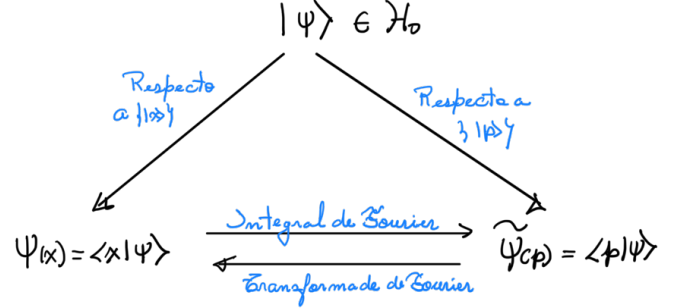
\includegraphics[scale=0.5]{img/transformadaFourier.png}
    \caption{Relación entre la base y la trasnformación usada para cambiar la función de estado de esta.}
    \label{fig:fourier}
\end{figure}

\begin{description}
    \item[Propiedad 14: ] $\mel{p}{X}{\psi} = i\hbar \displaystyle\pdv{\psim}{p}$. 
\end{description}



\section{Posición y Momentum 3-D}
Ahora estudiaremos los Observables de poisición y momentum en 3 dimensiones. Ya sabemos que la posición de las partículas está dada por $\vec{r} = (x,y,z)$ y $\vec{X} = (X,Y,Z)$.
\begin{tcolorbox}
        $$ X \ket{\vec{r}} = X \ket{\vec{x}} = X\ket{x,y,z} = x\ket{x,y,z} $$
        $$ Y \ket{\vec{r}} = Y \ket{\vec{y}} = Y\ket{x,y,z} = y\ket{x,y,z} $$
        $$ Z \ket{\vec{r}} = Z \ket{\vec{z}} = Z\ket{x,y,z} = z\ket{x,y,z}. $$
    También
        $$ \ket{\vec{r}} = \ket{x,y,z} = \ket{x} \ten \ket{y} \ten \ket{z} $$
        $$ \hilbert _1 = \hilbert _o \ten \hilbert _o \ten \hilbert _o. $$
\end{tcolorbox}
El conjunto de kets propios $\{ \ket{x,y,z} \}$ forma una base ortonormal $\hilbert _1$. Debido a que $\ket{\vec{x}}$ es una base ortonormal de $\hilbert _1$ tenemos que
    $$ \braket{\vec{x}}{\vec{x}'} = \delta ' (\vec{x} - \vec{x}'). $$
   

\subsection{Representación Respecto a $\{ \ket{\vec{x}} \}$}
Supongamos que la partícula está en el estado $\ket{\psi}\in \hilbert _1$. El ket $\pk$ se puede escribir como una superposición de los estados base.
    $$ \pk = \int _{\R ^3} \dd{^3  \vec{x}} \psi (\vec{x} \ket{\vec{x}}). $$
Debido a que $\{ \ket{\vec{x}} \}$ es una base ortonormal
    $$ \psi (\vec{x}) = \braket{\vec{x}}{\psi}. $$

\begin{description}
    \item[Propiedad 15: ] $[X_i ,X_j] = 0$ para $i,j = 1,2,3$. 
    \item[Propiedad 16: ] Siguiendo con la idea del operador traslación, tomando $a = \vec{a}$: $T_{\vec{a}}$ es unitario.
    \item 
\end{description}


\begin{definition}
    \textbf{Operador $P_j$:} \\
        $$ P_j = i\hbar \eval{\dv{T_{\vec{a}}}{a_j}} _{a_j = 0}. $$
    De esta definición se tiene
        $$ \mel{\vec{x}}{P_x}{\psi} = -i\hbar \pdv{\psi}{x} \qquad j = 1 $$
        $$ \mel{\vec{x}}{P_y}{\psi} = -i\hbar \pdv{\psi}{y} \qquad j = 2 $$
        $$ \mel{\vec{x}}{P_z}{\psi} = -i\hbar \pdv{\psi}{z} \qquad j = 3. $$
\end{definition}


\begin{description}
    \item[Propiedad 17: ] $[P_j,P_k] = 0 $.
    \item[Propiedad 18: ] $T_{\vec{a}} = e^{-\frac{i}{\hbar} \vec{a} \cdot \vec{P}}.$ 
    \item[Propiedad 19: ] Si $\vec{P} = (P_x,P_y,P_z)$ entonces
        $$ \mel{\vec{x}}{\vec{P}}{\psi} = -i\hbar \grad{\psi (\vec{x})}, $$
    donde $\psi (\vec{x}) = \braket{\vec{x}}{\psi}$.
    \item[Propiedad 20: ] Dado el momentum lineal total $P^2 = P_x ^2 + P_y ^2 + P_z ^2$. Entonces $\mel{\vec{x}}{P^2}{\psi} = -\hbar ^2 \laplacian{\psi}$.
    \item[Propiedad 21: ] $[X_j, P_k] = i\hbar \delta _{jk} I$. 
    \item[Propiedad 22: ] $[X_j ,P_j ^n] = i\hbar n P^{n - 1}$.
    \item[Propiedad 23: ] Sean $A,B,C$ operadores y $b,c$ números complejos.
        $$ [A,bB + cC] = b[A,B] + C[A,C]. $$
    \item[Propiedad 24: ] Sea $F(P_j) = \sum _{n=0} ^\infty a_n P_j ^n$ entocnes
        $$ [X_j ,F(P_j)] = i\hbar F' (P_j). $$
\end{description}


\section{Momentum Respecto a la Posición en 3-D}
El observable $\vec{P}$ es una terna ordenada (como era de esperarse luego de todo lo visto anteriormente) y son compatibles. Estos observables nos proporcionan una base ortonormal de nuestro espacio de estado. 

\begin{tcolorbox}
        $$ P_x \ket{\vec{p}} = P_x \ket{p_x,p_y,p_z} = p_x \ket{p_x,p_y,p_z} $$
        $$ P_y \ket{\vec{p}} = P_y \ket{p_x,p_y,p_z} = p_y \ket{p_x,p_y,p_z} $$
        $$ P_z \ket{\vec{p}} = P_z \ket{p_x,p_y,p_z} = p_z \ket{p_x,p_y,p_z}. $$
    También
        $$ \hilbert _1 = \hilbert _o \ten \hilbert _o \ten \hilbert _o. $$
\end{tcolorbox}

Sabemos
	$$ \psi (\vec{x}) = \braket{\vec{x}}{\psi}, $$
	$$ \psim (\vec{p}) = \braket{\vec{p}}{\psi}. $$

\begin{description}
	\item[Propiedad 25: ] $\braket{\vec{x}}{\vec{p}} = N e^{\frac{i}{\hbar} \vec{p} \cdot \vec{x}}$ Donde $N$ es una constante de normalización y $\vec{p} \cdot \vec{x} = xp_x + yp_y + zp_z$.
	\item[Propiedad 26: ] $\braket{\vec{x}}{\vec{p}} = \frac{1}{\qty(2\pi \hbar)^{3/2}} e^{\frac{i}{\hbar} \vec{p} \cdot \vec{x}}$.
	\item[Propiedad 27: (Transformada inversa de Fourier)] 
		$$ \psi (\vec{x}) = \frac{1}{\qty(2\pi \hbar)^{3/2}} \int _{\R^3} \dd{^3 \vec{p}} e^{\frac{i}{\hbar} \vec{p} \cdot \vec{x}} \psim (\vec{p}). $$
	\item[Propiedad 28: (Transformada de Fourier)] 
		$$ \psim (\vec{p}) = \frac{1}{\qty(2\pi \hbar)^{3/2}} \int _{\R^3} \dd{^3 \vec{p}} e^{-\frac{i}{\hbar} \vec{p} \cdot \vec{x}} \psi (\vec{x}). $$
\end{description}


\begin{definition}
	\textbf{Valor Propio Degenerado: } \\
	Sea $A:\hilbert \to \hilbert$ un opeardor lineal $a\in \C$ es un valor propio degenerado si y solo si existen vectores $\pk$ y $\ket{\phi}$ linealmente independientes tal que 
		$$ A\pk = a\pk $$
		$$ A\ket{\phi} = a\ket{\phi}. $$
	Recordemos del álgebra lineal que el conunto de todos los vectores propios de $A$ con valor propio $a$, forma un subespacio vectorial. De lo anterior tenemos que $a$ es un valor propio degenerado si y solamente si el espacio propio tiene dimensión mayor o igual a $2$.
\end{definition}


\begin{description}
	\item[Propiedad 29: ] Si $A$ y $B$ son observalbes que tienen la misma base ortonoral de kets porpios, entonces $A$ y $B$ son compatibles.
	\item[Propiedad 30: ] Si $A$ y $B$ son observables compatibles, donde todos sus valores propios son no degenerados, entonces $A$ y $B$ comparten base ortonormal de kets propios.
\end{description}

\begin{teorema}
	Si $A$ y $B$ son observables compatibles entonces $A$ y $B$ comparten base de kets propios.
\end{teorema}







\chapter{Energía y Hamiltoniano}

\section{Dinámica Cuántica}
Ahora se estudiará la evolución en el tiempo de un sistema cuántica. Dicho de otra forma, vamos a estudiar la evolución de un estado $\pk$ que representa un sistema interactuando con el medio.

\subsection{Operador Evolución $U(t,a)$}
El opeardor evolución describe el estado de un sistema después de haber transcurrido un tiempo $\Delta t=a$; de la siguiente forma
	$$ E(t,a) \Pk{t} = \Pk{t+a}. $$
El problema recae en calcular $U$.

\begin{description}
	\item[Propiedad 1: ] $U_a$ es unitario.
\end{description}


\section{El Hamiltoniano}
Ahor a definimos el Hamiltoniano en el tiemo $t$ de la sigueinte forma
	$$ H(t) = i\hbar \eval{\pdv{U(t,a)}{a}}_{a=0}. $$
Tal y como se verá más adelante $H$ es un operador Hermítico.

\begin{description}
	\item[Propiedad 2 (Ecuación de Schrodinger): ] $H(t) \Pk{t} = i\hbar \pdv{t} \Pk{t}$. Donde $H(t)$ es la energía total del sistema cuántico.
	\item[Propiedad 3: ] $H^+ (t) \Pk{t} = i\hbar \pdv{t} \Pk{t}$.
	\item[Propiedad 4: ] \dsnote{Ahora es bastante obvio}. $H$ es hermítico.
	 
\end{description}


\subsection{Casos del Hamiltoniano en Física}
En Física tenemos tres casos del Hamiltoniano
\begin{enumerate}
	\item El Hamiltoniano es independiente del tiempo
		$$ H(t) = H = \text{cte}. $$
	\item El Hamiltoniano depende del tiempo pero el Hamiltonianos a tiempos diferentes conmutan.
	\item El Hamiltoniano depende del tiempo y Hamiltonianos a tiempos diferentes no conmutan.
\end{enumerate}



\begin{description}
	\item[Propiedad 5: ] Si $H(t) = H$ es independiente del tiempo entonces.
		$$ U(t,a) = e^{-\frac{ia}{\hbar} H}. $$ 
	\item[Propiedad 6: ] Si los Hamiltonianos conmutan a tiempos diferentes
		$$ U(t,a) = e^{-\frac{i}{\hbar} \int _t ^{t+a} H(t') \dd{t'}}. $$
\end{description}


\section{Estados Estacionarios}
Recordemos que un estado se representa por un ket y cualquier múltiplo $c\pk$ representa el mismo estado. Un estado es estacionario si y solo si los kets $\Pk{t}$ que representan al estado del sistema en el tiempo $t$ son múltiplos de $\ket{\psi _o} = \Pk{0}$ para cualquier $t$, $\Pk{t} = c(t) \ket{\psi _o}$. \\

Los estados estacionarios no cambian respecto al tiempo, aunque los kets que los representan pueden cambiar. Siempre requerimos que la magnitud de los kets sea $1$ por lo tanto $c(t) = 1$. 
	$$ \Pk{t} = e^{i\theta (t)} \ket{\psi _o}. $$


Sea $A$ un observable cualquiera; el valor esperado del observable $A$ cuando el sistema está en el estado $\Pk{t}$ viene dado por:
\subsection{Punto de Vista de Heisenberg}
	$$ \expval{A} = \expval{\qty(U^+ (t) A U (t))}{\psi (0)}. $$
Para Heisenberg, el estado no evoluciona si no que evoluciona el observable.

	$$ A(t) = U^+ (t) AU(t). $$
	
\subsection{Punto de Vista de Schrodinger}
	$$ \expval{A(t)} = \qty(\bra{\psi (0)} U^+ (t)) A \qty(U(t) \Pk{t}). $$

Para Schrodinger, el observable no evoluciona sino que es el estado lo que evoluciona. Donde dicho estado obedece la ecuación de Schrodinger. \\
La ecuación de Schrodinger independiente del tiempo calcula los valores propios y kets propios del Hamiltoniano $H$.

\begin{description}
	\item[Propiedad Previa a la Ecuación de Heisenberg: ] 
		$$ \pdv{U(t)}{t} = \dv{U}{t} = \frac{1}{i\hbar} HU(t). $$ 
\end{description}


\subsection{Ecuación de Movimiento de Heisenberg}
Sea $A$ un observable y $H$ el Hamiltoniano.
	$$ \dv{A}{t} = \frac{1}{i\hbar} [A(t),H(t)]. $$





\chapter{Oscilador Armónico Cuántico}
El oscilador armónico cuántico es el análogo mecánico cuántico del oscilador armónico clásico. Es uno de los sistemas modelo más importante en mecánica cuántica, ya que cualquier potencial se puede aproximar por un potencial armónico en las proximidades del punto de equilibrio estable (mínimo). Además, es uno de los sistemas mecánico cuánticos que admite una solución analítica sencilla.


\section{Oscilador Armónico}
Dado el sistema físico de oscilador más simple se tiene que su hamiltoniano es
	$$ H = \frac{P^2}{2m} + \frac{1}{2} kX^2. $$
Dado que $H,P,X$ son observables incompatibles. Recordemos que $[X,P] = i\hbar I$. Y con esto tenemos el operador evolución
	$$ U(t) = e^{-\frac{i}{\hbar} tH}. $$


\section{Ecuación de Schrodinger}
	$$ H\pkt = i\hbar \pdv{t} \pkt $$
Si presentamos la ecuación de Schrodinger respecto a la posición, tenemos lo siguiente
	$$ -\frac{\hbar ^2}{2m} \pdv[2]{\Psi}{x} + \frac{m\omega ^2}{2} x^2 \Psi (x,t) = i\hbar \pdv{\Psi}{t}. $$

\subsection{Ecuación de Schrodinger Independiente del Tiempo}
La ecuación de Schrodinger independiente del tiempo es la ecuación que calcula los valores propios y los kets propios del Hamiltoniano mostrado al inicio del capítulo.
	$$ H\pk = E\pk, $$
$E$ es el valor propio de $H$, por lo tanto $E$ es un valor real puro, $E\in \R$.  Con esto aplicamos el bra $\bra{\psi}$ se llega a la ecuación de Schrodinger Independiente del Tiempo para el oscilador armónico, respecto a la posición
	$$ -\frac{\hbar ^2}{2m} \dv{\psi}{x} + \frac{m\omega ^2}{2} x^2 \psi (x) = E\psi (x). $$


\section{Operadores en el Oscilador Cuántico}
En lugar de resolver la ecuación de Schrodinger independiente del tiempo directamente, para calcular los valore propios y kets propios del Hamiltoniano; vamos a usar el operador creador, el operador anulador y el operador número. Como veremos a continuación el método de operadores es un método muy eficiente para calcular valores propios y ket propios.

\subsection{Operador Anulador o Aniquilador}
	$$ a = \sqrt{\frac{m\omega}{2\hbar}} \qty(X + i\frac{P}{m\omega}). $$


\subsection{Operador Creador}
	$$ a^\dagger = \sqrt{\frac{m\omega}{2\hbar}} \qty(X - i\frac{P}{m\omega}). $$
	
\subsection{Operador Número}
	$$ N = a^\dagger a. $$
	
Los operadores anulador y creador son operadores tipo escalera; no son ni hermíticos ni unitarios.



\subsection{Propiedades de los Operadores}

\begin{description}
	\item[Propiedad 1: ] $[a,a^\dagger] = I$.
	\item[Propiedad 2: ] $N = \frac{1}{\hbar \omega} H - \frac{1}{2} I$.
	\item[Propiedad 3: ] $H$ es hermítico.
	\item[Propiedad 4: ] $H$ y $N$ conmutan.
	\item[Propiedad 5: ] Si $\ket{n}$ es ket propio de $N$ con valor propio $n$ entonces
		$$ H\ket{n} = \qty(n + 1/2) \hbar \omega \ket{n}. $$
	\item[Propiedad 6: ] $[N,a] = -a$.
	\item[Propiedad 7: ] $[N,a^\dagger] = a^\dagger$.
	\item[Propiedad 8: ] $a\ket{n} = \sqrt{n} \ket{n - 1}$.
	\item[Propiedad 9: ] $a^\dagger \ket{n} = \sqrt{n + 1} \ket{n + 1}$.
	\item[Propiedad 10: ] Si $n$ es valor propio del operador número $N$ entonces $n\geq 0$.
	\item[Propiedad 11: ] Si $n$ es valor propio del operador número $N$ entonces $n$ es un número entero no negativo. 
	\item[Propiedad 12: ] Los valores y vectores propios de $N$ y $H$ son
		$$ H\ket{n} = \hbar \omega (n + 1/2) \ket{n}, $$
		$$ N\ket{n} = n\ket{n}. $$
	Dado esto vemos que la base ortonormal dada por el operador número y el hamiltoniano está discretizada. De esto se tiene que todo estado del oscilador armónico simple se puede escribir como una combinacion lineal de los estados propios de la energía total.
		$$ \pk = \sum _{n=0} ^\infty c_n \ket{n}. $$
	por fourier $C_n \braket{n}{\psi}$, amplitud de probabilidad de medir energía $\hbar \omega (n + 1/2)$ cuadno el sistema está en el estado $\pk$.
	\item[Propiedad 13: ] $\abs{c_n} ^2$ probabilidad de medir la energía $\hbar \omega (n + 1/2)$ cuando el sistema está en el estado $\pk$. \dsnote{Tarde vos pero $\ket{n}$ es el nivel de energía.}
\end{description}




Para continuar con todo esto, se calculará $\braket{x}{n}$ donde $\abs{\braket{x}{n}}^2$ es la probabilidad de medir la posición $x$ cuando la partícula está en el $n-$ésimo nivel de energía. Pero antes, más propiedades!!!!!


\begin{description}
	\item[Propiedad 14: ] $\ket{n} = \frac{1}{\sqrt{n!}} \qty(a^\dagger) ^n \ket{0}$.
	\item[Propiedad 15: ] Representación matricial de $a$: $\mel{l}{a}{n} = \sqrt{n} \delta _{l,n-1}$.
		$$ a = =
\begin{pmatrix}
0 & \sqrt{1} & 0 & 0 & \cdots \\
0 & 0 & \sqrt{2} & 0 & \cdots \\
0 & 0 & 0 & \sqrt{3} & \cdots \\
0 & 0 & 0 & 0 & \cdots \\
\vdots & \vdots & \vdots & \vdots & \ddots
\end{pmatrix} $$
	\item[Propiedad 16: ] Representación matricial de $a^\dagger$: $\mel{l}{a^\dagger}{n} = \sqrt{n + 1} \delta _{l,n+1}$.
		$$ a^\dagger = \begin{pmatrix}
0 & 0 & 0 & 0 & \cdots \\
\sqrt{1} & 0 & 0 & 0 & \cdots \\
0 & \sqrt{2} & 0 & 0 & \cdots \\
0 & 0 & \sqrt{3} & 0 & \cdots \\
0 & 0 & 0 & \sqrt{4} & \cdots \\
\vdots & \vdots & \vdots & \vdots & \ddots
\end{pmatrix} $$
	\item[Propiedad 17: ] $X = \sqrt{\dfrac{\hbar}{2m\omega}} (a + a^\dagger)$.
	\item[Propiedad 18: ] $P = i\sqrt{\dfrac{m\omega \hbar}{2}} (a^\dagger - a)$.
	\item[Propiedad 19: ] Representación matricial de $X$: $\mel{l}{X}{n} = \sqrt{\dfrac{\hbar}{2m\omega}} \qty(\sqrt{n} \delta _{l,n-1} + \sqrt{n+1} \delta _{l,n+1})$.
		$$ X = \sqrt{\frac{\hbar}{2m\omega}}
\begin{pmatrix}
0 & \sqrt{1} & 0 & 0 & \cdots \\
\sqrt{1} & 0 & \sqrt{2} & 0 & \cdots \\
0 & \sqrt{2} & 0 & \sqrt{3} & \cdots \\
0 & 0 & \sqrt{3} & 0 & \cdots \\
0 & 0 & 0 & \sqrt{4} & \cdots \\
\vdots & \vdots & \vdots & \vdots & \ddots
\end{pmatrix} $$
	\item[Propiedad 20: ] Representación matricial de $P$: $\mel{l}{P}{n} = i\sqrt{\dfrac{m\omega \hbar}{2}} \qty(-\sqrt{n} \delta _{l,n-1} + \sqrt{n+1} \delta _{l,n+1})$.
		$$ P = i \sqrt{\frac{\hbar m \omega}{2}}
\begin{pmatrix}
0 & -\sqrt{1} & 0 & 0 & \cdots \\
\sqrt{1} & 0 & -\sqrt{2} & 0 & \cdots \\
0 & \sqrt{2} & 0 & -\sqrt{3} & \cdots \\
0 & 0 & \sqrt{3} & 0 & \cdots \\
0 & 0 & 0 & \sqrt{4} & \cdots \\
\vdots & \vdots & \vdots & \vdots & \ddots
\end{pmatrix}. $$
	\item[Propiedad 21: ] $\braket{x}{0} = \dfrac{1}{\pi ^{1/4} \lambda ^{1/2}} e^{-\frac{1}{2} \qty(x/\lambda)^2}$, donde $\lambda \sqrt{\frac{\hbar}{m\omega}}$ y $\omega = \sqrt{\frac{k}{m}}$.
	\item[Propiedad 22: ] Si $\braket{x}{\psi} = \psi (x)$ entonces $\mel{x}{\qty(X - \frac{i}{m\omega} P)^n}{\psi} = \qty(x - \lambda ^2 \dv{x})^n \psi (x)$.
	\item[Propiedad 23: ] $\braket{x}{n} = \dfrac{1}{\pi ^{1/4} \sqrt{n! 2^n} \lambda ^{n + 1/2}} \qty(x - \lambda ^2 \dv{x})^n e^{1\frac{1}{2} \qty(\frac{x}{\lambda})^2}. $
\end{description}


\section{Dinámica del Oscilador Armónico Cuántico}
Primero se estudiará desde el punto de vista de Schrodinger y luego desde el punto de vista de Heisenberg. Desde el punto de vista de Schrodinger, lo que evoluciona es el estado $\pkt$ o sea que $\pkt = U(t) \pkt$. Desde el punto de vista de Heisenberg, o que evoluciona son los observables; donde, $X(t) = U(t) ^\dagger X(0) U(t)$, así para todos los observables. Para el oscilador armónico $H$ es independiente del tiempo.

\subsection{Punto de Vista de Schrodinger}
El estado de la partícula en el tiempo $t$ queda descrita por el ket $\pkt$. Para el oscilador cuántico el Hamiltoniano $H = \frac{P^2}{2m} + \frac{1}{2} m\omega ^2 X^2$ es independiente del tiempo
	$$ \pkt = e^{-\frac{itH}{\hbar}} \ket{\psi _o}. $$
	
\subsection{Solución al Oscilador Armónico Cuántico}
Si el oscildor inicialmente está en el estado $\Pk{o}$ vamos a calcular su estado en el tiempo $t$, respecto a la base otorgada por el Hamiltoniano $\{ \ket{n} \}$.

\begin{description}
	\item[Propiedad 1: ] $e^{-\frac{it}{\hbar} H} \ket{n} = e^{-i\omega (n + 1/2) t} \ket{n}$. Entonces
		$$ \pkt = \sum _{n = 0} ^\infty b_n (t) \ket{n}, $$
	donde $b_n (t) = c_n e^{-in\omega t}$.
\end{description}



\subsection{Punto de Vista de Heisenberg}
Desde el punto de visa de Heisenberg el estado no evoluciona, los que evolucionan son los observables. Recordando 
	\begin{align*}
		X(t) &= U^\dagger (t) X U(t), \\
		P(t) &= U^\dagger (t) P U(t).
	\end{align*}

	\begin{align}
		\begin{array}{ccc}
			\dv{X}{t} & = & \frac{1}{i\hbar} [X(t) ,H(t)] \\
			 & & \\
			\dv{P}{t} & = & \frac{1}{i\hbar} [P(t) ,H(t)].
		\end{array} \text{ Ecuación de Heisenberg.}
	\end{align}
En el oscilador armónico cuántico $H(t) = H$. Desarrollando los conmutadores y utilizando propiedades de las aprendidas, se tiene que
	\begin{align}
		\dv{X}{t} &= \frac{P(t)}{m} \\
		\dv{P}{t} &= -m\omega ^2 X(t).
	\end{align}













\chapter{Espín $1/2$}
En este capítulo se estudiará un sistema cuántico con dos estados independientes, osea que el espacio de estado es un espacio de dos dimensiones, $\C ^2$. El experimento físico que motiva el formalismo es el experimento de Stern-Gerlach, el cual ya se mostró al inicio del capítulo $17$. 

\section{Generalidades}
De lo mostrado en esa explicación vamos a establecer que el ket propio para el espín con valor positivo $+\hbar /2$ es $\ket{S_z , +\hbar/2} = \ket{S_z, +} = \ket{+}$ y el otro ket propio es $\ket{S_z , -\hbar/2} = \ket{S_z, -} = \ket{-}$. Por lo tanto tenemos una base para el espacio de estado $\C^2$ que es $\alpha = \{ \ket{+},\ket{-} \}$. Osea que
	\begin{align}
		S_z \ket{+} &= \frac{\hbar}{2} \ket{+} \\
		S_z \ket{-} &= -\frac{\hbar}{2} \ket{-}.
	\end{align}

Entonces, el observable $S_z$ representado respecto a la base $\alpha$
	$$ \qty(S_z)_\alpha = \frac{\hbar}{2} \mqty(1 & 0 \\ 0 & -1). $$
Todoe stado de las partículas se representa por medio de un ket como una superposición de los kets propios del observable $S_z$
	$$ \pk = a\ket{+} + b\ket{-}. $$
donde siempre requerimos que $\abs{a} ^2 + \abs{b} ^2 = 1$.

\subsection{El Operador Identidad}
Recordemos que si $\alpha$ es base del espacio de estado $\hilbert$ entonces
	\begin{align}
		I = \ketbra{+} + \ketbra{-}.
	\end{align}


\subsection{Cambio de Base}
El aparato para observar $S_z$ cuando es girado nos da otro observable, en especial cuando lo giramos $90^o$. Tenemos otro observable qeu es $S_x$ y se obtienen solamente dos valores $\pm \frac{\hbar}{2}$, obteniendo otros dos kets propios que representan los kets propios del observable $S_x$
	\begin{align}
		S_x \ket{S_x,+} &= \frac{\hbar}{2} \ket{S_x, +} \\
		S_x \ket{S_x,-} &= \frac{\hbar}{2} \ket{S_x, -}.
	\end{align}
Entonces tenemos la siguiente observación del experimento
	\begin{align*}
		\abs{\braket{S_x,+}{S_z,+}}^2 &= \frac{1}{2} \\
		\abs{\braket{S_x,-}{S_z,+}}^2 &= \frac{1}{2}.
	\end{align*}
Recordemos que $\abs{\braket{S_x,+}{S_z,+}}^2$ es la probabilidad de medir $+\hbar /2$ en el eje $x$ cuando la partícula está en el estado $\ket{+}$. De lo anterior tenemos que $S_x$ y $S_z$ son incompatibles y dan bases diferentes de kets propios. A la base en el eje $x$ le llamaremos $\beta$.

\subsubsection{Representación de $\mathbf{\ket{S_x,\pm}}$ y $\mathbf{\ket{S_y, \pm}}$ respecto a $\mathbf{\alpha}$}
Vamos a calcular los siguientes valores para $a_{ij}$ y $b_{ij}$.
\begin{align*}
	\spinp{x} &= a_{11} \plus + a_{21} \minus \\
	\spinm{x} &= a_{21} \plus + a_{22} \minus
\end{align*}

además\footnote{a la base de $y$ le llamaremos $\gamma$.}

\begin{align*}
	\spinp{y} &= b_{11} \plus + b_{21} \minus \\
	\spinm{y} &= b_{21} \plus + b_{22} \minus
\end{align*}

Sujeto a las siguientes condiciones

\begin{align*}
	\abs{\braket{S_x, +}}^2 &= \abs{\braket{S_x, -}}^2 = 1 \\
	\abs{\braket{S_y, +}}^2 &= \abs{\braket{S_y, -}}^2 = 1
\end{align*}
Así como también $\braket{S_x,+}{S_x,-} = \braket{S_y,+}{S_y,-} = 0$. Y calculando los brakets se tiene que $\abs{a_{11}}^2 = \abs{a_{12}}^2 = \abs{a_{21}}^2 = \abs{a_{22}}^2 = \frac{1}{2}$. De lo anterior llegamos a
	$$ \spinp{x} = e^{i\phi} \qty(\frac{1}{\sqrt{2}} \plus + \frac{e^{i\phi _1}}{\sqrt{2}} \minus) $$
además, $\spinp{x} = e^{-i\phi} \spinp{x}$, representan el mismo estado, por lo tanto podemos elegir la fase igual a cero. Se hace lo mismo para $\spinm{x}$.
\begin{align}
	\spinp{x} &= \frac{1}{\sqrt{2}} \plus + \frac{e^{i\phi _1}}{\sqrt{2}} \minus \\
	\spinm{x} &= \frac{1}{\sqrt{2}} \plus - \frac{e^{i\phi _1}}{\sqrt{2}} \minus .
\end{align}
Y se realiza el mismo procedimiento para $\ket{S_y, \pm}$.

\begin{align}
	\spinp{y} &= \frac{1}{\sqrt{2}} \plus + \frac{e^{i\phi _3}}{\sqrt{2}} \minus \\
	\spinm{y} &= \frac{1}{\sqrt{2}} \plus - \frac{e^{i\phi _3}}{\sqrt{2}} \minus .
\end{align}

Reemplazando las fases se tiene

\begin{tcolorbox}
	\begin{align}
		\spinp{x} &= \frac{1}{\sqrt{2}} \plus + \frac{1}{\sqrt{2}} \minus \\
		\spinm{x} &= \frac{1}{\sqrt{2}} \plus - \frac{1}{\sqrt{2}} \minus \\
		\spinp{y} &= \frac{1}{\sqrt{2}} \plus + \frac{i}{\sqrt{2}} \minus \\
		\spinm{y} &= \frac{1}{\sqrt{2}} \plus - \frac{i}{\sqrt{2}} \minus .
	\end{align}
\end{tcolorbox}

Ahora, veremos matricialmente los observables respecto a la base $\alpha$. Ahora tenemos

\begin{tcolorbox}
	\begin{align}
		\plus &= \frac{1}{\sqrt{2}} \spinp{x} + \frac{1}{\sqrt{2}} \spinm{x} \\
		\minus &= \frac{1}{\sqrt{2}} \spinp{x} - \frac{1}{\sqrt{2}} \spinm{x} \\
		\plus &= \frac{1}{\sqrt{2}} \spinp{y} + \frac{1}{\sqrt{2}} \spinm{y} \\
		\minus &= -\frac{i}{\sqrt{2}} \spinp{y} + \frac{i}{\sqrt{2}} \spinm{y} .
	\end{align}
\end{tcolorbox}


\subsubsection{Representación Matricial de $S_x$ Respecto a $\alpha$}

Aplicamos el operador $S_x$ a los elementos dela base $\alpha$.

\begin{equation}
	(S_x)_\alpha = \frac{\hbar}{2} \mqty(0 & 1 \\ 1 & 0).
\end{equation}


Donde $\smqty(\pmat{1})$ es la \textbf{primera matriz de pauli} $\sigma _1 = \sigma _x$.






\subsubsection{Representación Matricial de $S_y$ Respecto a $\alpha$}

Aplicamos el operador $S_y$ a los elementos dela base $\alpha$.

\begin{equation}
	(S_y)_\alpha = \frac{\hbar}{2} \mqty(0 & -i \\ i & 0).
\end{equation}
Donde $\smqty(\pmat{2})$ es la \textbf{segunda matriz de pauli} $\sigma _2 = \sigma _y$.









\subsubsection{Representación Matricial de $S_z$ Respecto a $\alpha$}

Aplicamos el operador $S_z$ a los elementos dela base $\alpha$.

\begin{equation}
	(S_z)_\alpha = \frac{\hbar}{2} \mqty(1 & 0 \\ 0 & -1).
\end{equation}
Donde $\smqty(\pmat{3})$ es la \textbf{tercera matriz de pauli} $\sigma _3 = \sigma _z$.


\subsection{Matrices de Pauli}
Las matrices de pauli son matrices hermíticas que me sirven de base para formar un Espacio Vectorial sobre los reales que eventualmente se convertirá en un Álgebra de Lie.

\begin{equation}
	\pauli{x} = \mqty(\pmat{1}), \qquad \pauli{y} = \mqty(\pmat{2}), \qquad \pauli{z} = \mqty(\pmat{3}).
\end{equation}



\section{Espín Total $S^2$}
El espín total $S^2$ se define de la siguiente forma
\begin{equation}
	S^2 = S_x ^2 + S_y ^2 + S_z ^2.
\end{equation}


\begin{description}
	\item[Propiedad 1: ] $S^2 = \frac{3\hbar ^2}{4} I$.
\end{description}


\subsection{Operadores Escaleras $S_+,S_-$}
Tenemos que la base propia del observable $S_x$ es $\beta$ y la del observable $S_y$ es $\gamma$; estad dos bases son diferentes, lo que implican que son incompatibles, no se pueden medir simultaneamente. Debido a lo anterior vamos a definir los operadores escalera
	\begin{align}
		S_+ &= S_x + iS_y \\
		S_- &= S_x - iS_y,
	\end{align}
observemos que  $S_+ ^\dagger = S_-$ y vicebersa, no son operadores hermíticos, ni unitarios; son operadores tipo escalera.


\begin{description}
	\item[Propiedad 2: ] $S_+ = \hbar \ketbra{+}{-}$.
	\item[Propiedad 3: ] $S_- = \hbar \ketbra{-}{+}$.
	\item[Propiedad 4: ] 
		$$ S_x = \frac{1}{2} (S_x + S_-) $$
		$$ S_y = \frac{1}{2i} (S_x - S_-) $$
	\item[Propiedad 5: ] $[S_x ,S_y] = i\hbar S_z$.
\end{description}

\section{Preseción del Espín $1/2$}
En esta clase vamos a estudiar la evolucion del espín en un eletrón sometido a un campo magnético $\vec{B}$ uniforme y constante dirigido en la dirección $z$. Debido a que el electrón tiene estpín, también tiene un momento dipolar magnético $\vec{\mu}$; para el electrón $\mu = \frac{\hbar e}{2mc}$, donde $e$ es la carga del electrón. La dirección del momento dipolar magnético es la misma que la del espín. Además tenemos que al estar un electrón en un campo magnético $\vec{B}$ tenemos que la energía total es: $U = -\vec{\mu} \cdot \vec{B}$. Nosotros medimos el observable del espín por medio del momento dipolar magnético. Antes de plantear el hamiltoniano consideremos la siguiente expresión para el espín $\vec{S}$ que es el espín total, con esto tenemos el hamiltoniano
\begin{equation}
	H = \vec{\mu} \cdot \vec{B} = -\frac{e}{mc} \vec{S} \cdot \vec{B}.
\end{equation}

Considerando que el campo magnético está en la dirección del eje $z$: $H = -\frac{eB_z}{mc} S_z$. Tomando las constantes como un nuevo parámetro $\omega = -\frac{eB_z}{mc}$ $\Rightarrow$ $H = \omega S_z$.


\section{Evolución de un Estado}
Ahora vamos a estudiar la forma en que evoluciona un estado cualquiera $\Pk{o}$ sometido a un Hamiltoniano $H = \omega S_z$. Ahora
\begin{equation}
	U(t) = e^{-\frac{i\omega t}{\hbar} S_z}.
\end{equation}

\begin{description}
	\item[Propiedad 1: ] $e^{-\frac{i\omega t}{\hbar} S_z} \plus = e^{-\frac{i\omega t}{2}} \plus$.
	\item[Propiedad 2: ] $e^{-\frac{i\omega t}{\hbar} S_z} \minus = e^{\frac{i\omega t}{2}} \minus$.
\end{description}




\subsection{Casos Especiales}
Como primera instancia vamos a considerar que el estado inicial es un estado propio del Hamiltoniano $H = \omega S_z$ por ejemplo $H\plus = \frac{\omega \hbar}{2} \plus$.

\begin{description}
	\item[Caso 1: ($\Pk{o} = \plus$)] $\pkt = e^{-\frac{i\omega t}{2}} \plus$ pero eso representa el mismo estado que $\plus$. En este caso $\plus$ representa un estado estacionario. \dsnote{los kets del Hamiltoniano representan estados estacionarios que no evolucionan.} 
	\item[Caso 2: (Estado inicial $\spinp{x}$)] En este caso $\Pk{o} = \spinp{x}$ o sea que $\Pk{t} = \frac{1}{\sqrt{2}} \plus + \frac{e^{i\omega t}}{\sqrt{2}} \minus$. Valuando
		\begin{align*}
			\Pk{\pi /2\omega} &= \spinp{y} \\
			\Pk{\pi /\omega} &= \spinm{x} \\
			\Pk{3\pi / 2\omega} &= \spinm{y}
		\end{align*}
	El ''cono'' va precesando (rotando) con una velocidad angular de precesión igual a $\omega$.
\end{description}


\subsection{Consideraciones sobre el Espín $1/2$}
Aspectos del Espín $1/2$ que son las siguientes:
\begin{enumerate}
	\item Los estados del espín $1/2$ como ejemplo secillo de espinor.
	\item Entrelazamiento dos partículas, cada una de ellas con espín $1/2$.
\end{enumerate}

\subsubsection{Estados de Espín $1/2$ como Espinor}
REcordemos que estamos estudiando una partícula de espín $1/2$ cuyo espacio de estado es $\hilbert = \C^2$ que es un espacio unitario. En el espacio de estado $\hilbert$  tenemos un producto interno dado por el Braket. En otras palabras el espcio de estado tiene estructura geométrica llamada unitaria. POdemos hablar de ortogonalidad entre estados y magnitud de kets. 



\subsubsection{Entrelazamiento de dos Partículas con Espín $1/2$}
Vamos a considerar dos partículas, la partícula con espín $1/2$ y la partícula con espín $1/2$ también. Con estas dos partículas formamos un sistema de dos partículas de espín $1/2$ donde podemos medir el momentum anguloar total y el momentum angular en $z$. Dado el sistema de dos partículas su espacio de estado esta dado por $\hilbert = \hilbert _1 \ten \hilbert _2$ cuya base es $\{ \plus \ten \plus, \plus \ten \minus, \minus \ten \plus, \minus \ten \minus \} = \{ \ket{\upuparrows}, \ket{\updownarrows}, \ket{\downuparrows}, \ket{\downdownarrows} \}$. Vamos a medir el momentum angular del sistema en el eje $z$ 

\begin{align*}
	J_z \ket{\upuparrows} &= \hbar \upuparrows \\
	J_z \ket{\updownarrows} &= 0 \updownarrows \\
	J_z \ket{\downuparrows} &= 0 \downuparrows \\
	J_z \ket{\downdownarrows} &= -\hbar \downdownarrows
\end{align*}
$J_z$ es la adición\footnote{Adición de Espínes: $J_{i} = S_{1i} \boxplus S_{2i} = S_{1i} \ten I + I\ten S_{2i}$, con $i = \{ x,y,z \}$.} de $S_{1z}$ y $S_{2z}$
\begin{equation}
	J_z = S_{1z} \boxplus S_{2z}.
\end{equation}








\chapter{Momentum Angular}

\section{Introducción por Medio de los Observables del Spin}
Co lo último visto en el capítulo anterior, definimos un operador de momentum angular más general
	\begin{equation}
		J^2 = J_x ^2 + J_y ^2 + J_z ^2 .
	\end{equation}
La base de kets propios $\{ \ket{\upuparrows}, \ket{\updownarrows}, \ket{\downuparrows}, \ket{\downdownarrows} \}$ es base de $J_z$ pero no son kets propios de $J^2$. Ahora mostramos su representación matricial
\begin{align}
	J_x &= \frac{\hbar}{2} \mqty(0 & 1 & 1 & 0 \\
								 1 & 0 & 0 & 1 \\
								 1 & 0 & 0 & 1 \\
								 0 & 1 & 1 & 0), \\
	J_y &= \frac{\hbar}{2} \mqty(0 & -i & -i & 0 \\
								 i & 0 & 0 & -i \\
								 i & 0 & 0 & -i \\
								 0 & i & i & 0), \\
	J_z &= \hbar \mqty(1 & 0 & 0 & 0 \\
								 0 & 0 & 0 & 0 \\
								 0 & 0 & 0 & 0 \\
								 0 & 0 & 0 & -1), \\
	J^2 &= \hbar ^2 \mqty(2 & 0 & 0 & 0 \\
								 0 & 1 & 1 & 0 \\
								 0 & 1 & 1 & 0 \\
								 0 & 0 & 0 & 0).
\end{align}
Encontramos los kets propios de $J^2$, los cuales forman la siguiente base $\{ \ket{\upuparrows}, \frac{1}{\sqrt{2}} (\ket{\updownarrows} + \ket{\downuparrows}, \ket{downdownarrows}, \frac{1}{\sqrt{2}} (\ket{\updownarrows} - \ket{\downuparrows}) \}$.
\begin{equation}
	\qty(J^2)_\delta = \mqty(2\hbar ^2 & 0 & 0 & 0 \\
							 0 & 2\hbar ^2 & 0 & 0 \\
							 0 & 0 & 2\hbar ^2 & 0 \\
							 0 & 0 & 0 & 0).
\end{equation}


Recordemos el postulado 5: Cuando medimos un observable, el estado del sistema cambia (colapsa) a un estado propio del observable, correspondiente al valor propio que medimos.

\paragraph{Observación: }
Al medir el momentum angular total $J^2$ de un sistema de dos partículas con spín $1/2$ estas partículas quedan entrelazadas en estado propio correspondiente al valor propio que medimos. Cuando medimos $J^2$ obtenemos $2\hbar ^2$ o cero. Si medimos $2\hbar ^2$ para $J^2$ el sistema queda en algún estado generado por los kets propios correspondientes $\{ \ket{\upuparrows}, \frac{1}{\sqrt{2}} (\ket{\updownarrows} + \ket{\downuparrows}, \ket{downdownarrows}, \frac{1}{\sqrt{2}} (\ket{\updownarrows} - \ket{\downuparrows}) \}$. Pero si cuando medimos $J^2$ obtenemos cero el sistema de las dos partículas está en el estado 
	$$ \pk = \frac{1}{\sqrt{2}} \ket{\upuparrows} - \frac{1}{\sqrt{2}} \ket{\downdownarrows} $$
donde a los coeficientes se les conocen como \textbf{Coeficientes de Clebsh-Gordan}. Si estamos en el estado $\pk$ y a continuación medimos $S_{1z}$ podríamos obtener $\pm \frac{\hbar}{2}$. Un resultado del entrelazamiento es el siguiente:




\begin{tcolorbox}
	Si medimos $S_{1z}$ cuando el sistema está en el estado $\pk$ y nos da $+\hbar /2$ entonces con toda seguridad al medir $S_{2z}$ nos dará $-\hbar /2$. SI medimos $S_{1z}$ cuando el sistema está en el estado $\pk$ y nos da $-\hbar /2$ entonces con toda seguridad al medir $S_{2z}$ nos dará $+\hbar /2$.
\end{tcolorbox}


\section{Introducción Formal}
Recordando como se definió el momentum lineal, usamos traslaciones en espacios euclideanos. De forma análoga vamos a usar rotaciones en espacios euclideanos para introducir el concepto de momentum angular.


\subsection{Rotación Pasiva}
\dsnote{No lo voy a decir...} Es la clásica: (se rotan los ejes de referencia)

$$ \mqty(x' \\ y' \\ z') = \mqty(\cos \alpha & \sen \alpha & 0 \\ -\sen \alpha & \cos \alpha & 0 \\ 0 & 0 & 1) \mqty(x \\ y \\ z). $$
Rotación $R_z (\alpha)$ ángulo $\alpha$ alrededor del eje $z$.

\subsection{Rotación Activa}
Se rota el objeto, no rota el sistema de referencia.

$$ \mqty(x' \\ y' \\ z') = \mqty(\cos \alpha & -\sen \alpha & 0 \\ \sen \alpha & \cos \alpha & 0 \\ 0 & 0 & 1) \mqty(x \\ y \\ z). $$
Por el momento se le dará preferencia al punto de vista activa, con el cual vamos a desarrollar la teoría básica del Momentum Angular.

\begin{description}
	\item[Propiedad 1: ] $D_z (\alpha)$ es un operador unitario.
	\item[Propiedad 2: ] $\mel{r,\theta ,\phi}{D_z (\alpha)}{\psi}$
\end{description}


\section{Operadores}

\subsection{Definición del Operador $L_z$}
\begin{equation}
	L_z = i\hbar \eval{ \dv{D_z (\alpha)}{\alpha} }_{\alpha = 0}.
\end{equation}


\begin{description}
	\item[Propiedad 3: ] $\mel{r,\theta, \phi}{L_z}{\psi} = -i\hbar \pdv{\psi (r,\theta,\phi)}{\phi}$.
	\item[Propiedad 4: ] $\mel{r,\theta ,\phi}{\qty(\frac{\alpha L_z}{i\hbar})^n}{\psi} = \qty(-\alpha)^n \pdv[n]{\psi}{\phi}.$
	\item[Propiedad 5: ] $D_z (\alpha) = e^{-\frac{i\alpha L_z}{\hbar}}$.
	\item[Propiedad 6: ] $\mel{r,\theta ,\phi}{L_z ^\dagger}{\psi} = -i\hbar \pdv{\psi}{\phi}$. Lo que implica que $L_z ^\dagger = L_z$ es Hermítico.
	\item[Propiedad 7: ] Calculamos los operadores en términos de los observables de posición y momentum.
			\begin{align}
				L_z &= XP_y - YP_x \\
				L_x &= YP_z - ZP_y \\
				L_y &= ZP_x - XP_x 
			\end{align}
		y
			\begin{align*}
				D_x (\alpha) &= e^{-\frac{i\alpha L_x}{\hbar}} \\
				D_y (\alpha) &= e^{-\frac{i\alpha L_y}{\hbar}}
			\end{align*}
		A diferencia de las traslaciones, las rotaciones no conmutan.
\end{description}


\section{Momentum Angular Orbital}
Tomando el producto cruz como se definió en kinder, definimos el momentum angular orbital se tiene
\begin{equation}
	\vec{L} = \vec{R} \cp \vec{P}.
\end{equation}


\begin{description}
	\item[Propiedad 8: ] Conmutadores.
		\begin{align}
			[L_x ,L_y] &= i\hbar L_z \\
			[L_x ,L_z] &= -i\hbar L_y \\
			[L_y ,L_z] &= i\hbar L_x .
		\end{align}
	\item[Propiedad 9: ] Dado el momentum angular total $L^2 = L_x ^2 + L_y ^2 + L_z ^2$, se tiene $[L^2 ,L_k] = 0$, con $k = \{ x,y,z \}$.
	\item[Propiedad 10: ] Operadores escalera
		\begin{align*}
			L_+ &= L_x + iL_y \\
			L_- &= L_x - iL_y.
		\end{align*}
\end{description}

\subsection{Valores y Vectores Propios}
\begin{align}
	L_z \ket{i,m} &=m\hbar \ket{j,m} \\
	L^2 \ket{j,m} &= \lambda _j \ket{j,m} .
\end{align}


\begin{description}
	\item[Propiedad 11: ] $[L_+ ,L_-] = 2\hbar L_z$.
	\item[Propiedad 12: ] $[L_z ,L_+] = \hbar L_+$ y $[L_z ,L_-] = -\hbar L_-$.
	\item[Propiedad 13: ] $L^2 = \frac{1}{2} \qty(L_+ L_- + L_- L_+) + L_z ^2$.
	\item[Propiedad 14: ] $L^2 = L_z ^2 + \hbar L_z + L_- L_+$ y $L^2 = L_z ^2 - \hbar L_z + L_+ L_-$.
	\item[Propiedad 15: ] Ahora, volviendo al operador general de momento angular
		\begin{align*}
			J_+ &= J_x + iJ_y \\
			J_- &= J_x - iJ_y \\
			[J_+ ,J_-] &= 2\hbar J_z \\
			[J_z ,J_+] &= \hbar J_+ \\
			[J_z ,J_-] &= -\hbar J_- \\
			J &= \frac{1}{2} \qty(J_+ J_- + J_- J_+) + J_z ^2 \\
			J^2 &= J_z ^2 - \hbar J_z + J_+ J_-.
		\end{align*}
	\item[Propiedad 16: ] $L_+ \ket{j,m} = c\ket{i,m+1}$.
	\item[Propiedad 17: ] $L_- \ket{j,m} = c\ket{j,m-1}$.
	\item[Propiedad 18: ] $L^2 \ket{j,m} = \hbar ^2 j(j + 1) \ket{j,m}$.
	\item[Propiedad 19: ] Elvalor mínimo de $m$ para los kets propios $\ket{j,m}$ con $j$ fijo es $m=-j$.
	\item[Propiedad 20: ] Los valores que puede tener $j$ son los siguietnes $j = 0, 1/2, 1, 3/2, 2, 5/2, \ldots$.
	\item[Propiedad 21: ] Dimensión del subespaio propio para $j$: dim$\hilbert _j = 2j+1$.
	\item[Propiedad 22: ] $L_+ \ket{j,m} = \hbar \sqrt{j(j+1) - m(m + 1)} \ket{j,m + 1}$.
	\item[Propiedad 23: ] $L_- \ket{j,m} = \hbar \sqrt{j(j+1) - m(m - 1)} \ket{j,m - 1}$.
\end{description}


\subsection{Armónicos Esféricos}
La representación delos ket propios $\ket{l,m}$, cuando $l$ es entero, respecto a la posición en coordenadas esféricas nos quedan los Armónicos Esféricos. Ahora $l=0,1,2,\ldots$
	\begin{equation}
		\braket{r,\theta ,\phi}{l,m} = Y_l ^m (\theta ,\phi).
	\end{equation}





\chapter{Métodos Aproximados}











\chapter{Problemas en Una Dimensión}





















%%%%